\section{Conductores Paralelos}%
\label{sec:conductores_paralelos}
Las primeras simulaciones consistieron en simular el acoplamiento entre dos conductores paralelos, con y sin blindaje. Las frecuencias de simulación se encontraron en dos rangos: uno en el que la longitud eléctrica de los conductores permite trabajar con un modelo de parámetros concentrados, y otro en el que los conductores son eléctricamente largos, por lo que es necesario trabajar con un modelo de líneas de transmisión y radiación.
Para las simulaciones en bajas frecuencias, el acople se explica por efectos capacitivos e inductivos entre los conductores, que pueden ser expresados por un modelo de parámetros concentrados. En particular, puede modelarse el acople con capacidades a tierra, capacidad entre los conductores e inductancia mutua entre los conductores. En altas frecuencias, el acople se explica con un modelo que contemple los efectos de radiación de las líneas.
Todas las simulaciones se realizaron con el programa \textit{FEKO}.

\subsection{Conductores sin Blindaje}%
\label{sub:conductores_sin_blindaje}

En la figura Figura~\ref{fig:imagenes/conductores_sin_blindaje_simulacion} podemos ver la estructura de la simulación de los conductores sin blindaje. Todos los parámetros de interés se guardaron como variables para poder variar la simulación con facilidad. La simulación consistió en excitar un conductor con una fuente, y obtener la respuesta en el puerto opuesto del otro conductor. Los resultados se le solicitaron al programa en forma de parámetros S.

\begin{figure}[ht]
  \centering
  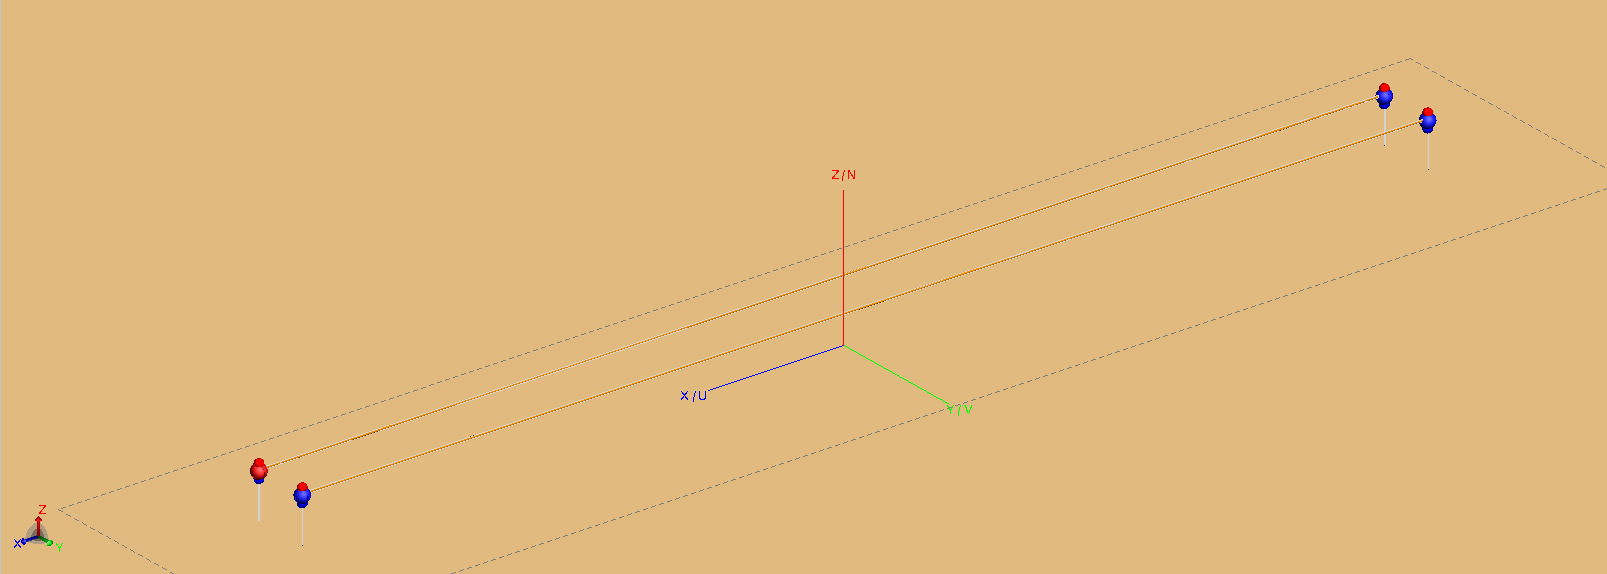
\includegraphics[width=0.8\linewidth]{imagenes/conductores_sin_blindaje_simulacion.png}
  \caption{Simulación de conductores sin blindaje}%
  \label{fig:imagenes/conductores_sin_blindaje_simulacion}
\end{figure}

\subsection{Conductores con Blindaje}%
\label{sub:conductores_con_blindaje}

La construcción de la simulación de los conductores con blindaje fue idéntica a la de los conductores sin blindaje: se parametrizaron todas las variables, se solicitaron parámetros S. La única diferencia fue que el conductor victima del acoplamiento fue rodeado de un blindaje de \SI{7}{\mm} de radio. En la figura~\ref{fig:imagenes/conductores_con_blindaje_simulacion} vemos la simulación.

\begin{figure}[ht]
  \centering
  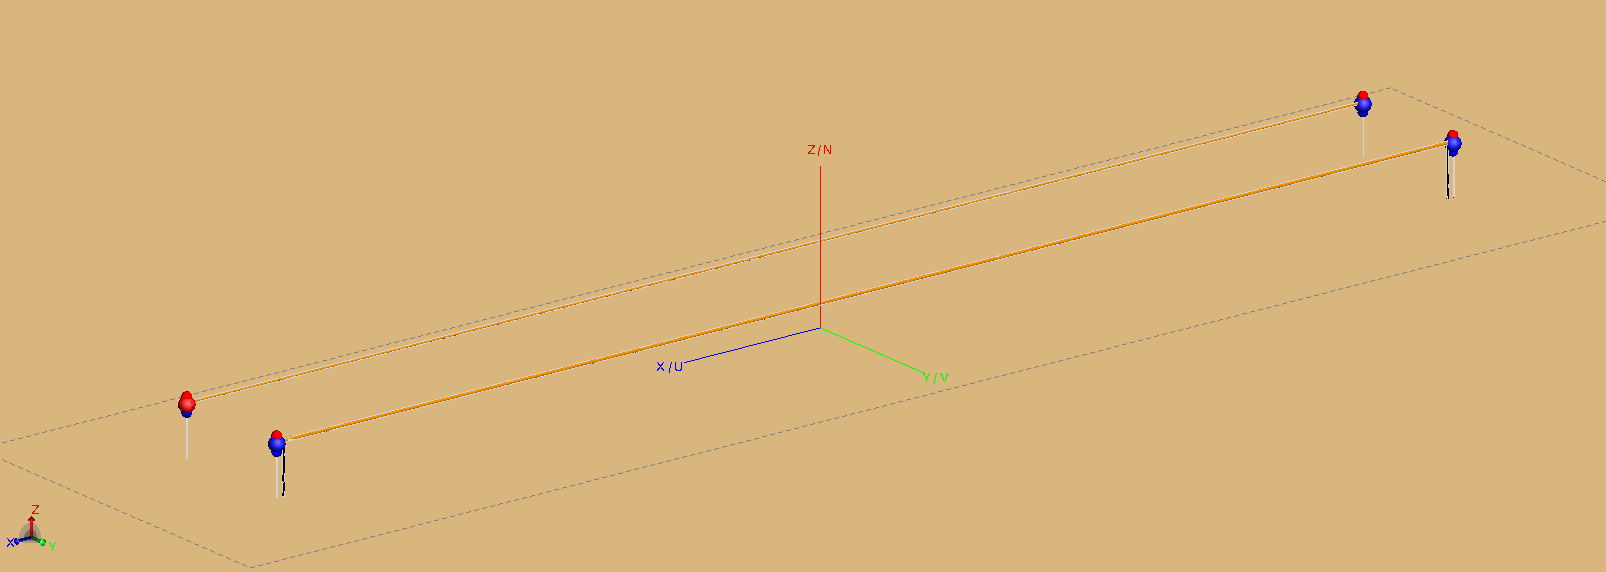
\includegraphics[width=0.8\linewidth]{imagenes/conductores_con_blindaje_simulacion.png}
  \caption{Simulación de conductores con blindaje}%
  \label{fig:imagenes/conductores_con_blindaje_simulacion}
\end{figure}

\subsection{Resultados}%
\label{sub:resultados_conductores}

En las figuras ~\ref{fig:imagenes/acoplamiento_sin_blindaje_resultados_bajas} a ~\ref{fig:imagenes/acoplamiento_con_blindaje_resultados_altas} podemos ver los resultados de las simulaciones descriptas anteriormente. Comentamos lo siguiente

\begin{itemize}
  \item En la figura ~\ref{fig:imagenes/acoplamiento_sin_blindaje_resultados_bajas} vemos los resultados del acoplamiento para conductores sin blindaje, para distintas separaciones. Podemos ver el efecto de la separación en el acoplamiento, que representa una diferencia de aproximadamente \SI{15}{\dB}. En la figura ~\ref{fig:imagenes/acoplamiento_con_blindaje_resultados_bajas} vemos el mismo resultado para conductores sin blindaje. La variación con la distancia es la misma, pero el acoplamiento baja en aproximadamente \SI{20}{\dB}.
  \item Podemos ver los efectos del blindaje en las figuras ~\ref{fig:imagenes/efecto_blindaje_25cm} y ~\ref{fig:imagenes/efecto_blindaje_50cm}. Vemos que con blindaje, el acoplamiento cae en aproximadamente \SI{20}{\dB}, para las separaciones de \SI{25}{\cm} y \SI{50}{\cm}.
  \item En las figuras ~\ref{fig:imagenes/acoplamiento_sin_blindaje_resultados_altas} y ~\ref{fig:imagenes/acoplamiento_con_blindaje_resultados_altas} podemos ver los efectos del acople para altas frecuencias, donde no se cumple la aproximación cuasi estática. Vemos que el acoplamiento tiene una respuesta debida a un modelo de altas frecuencias, en el que las líneas son eléctricamente largas y se ven sometidas a efectos de radiación y acople por radiación. Hay picos debido a frecuencias en las que las longitudes hacen al sistema resonante.
\end{itemize}

\begin{figure}[ht]
  \centering
  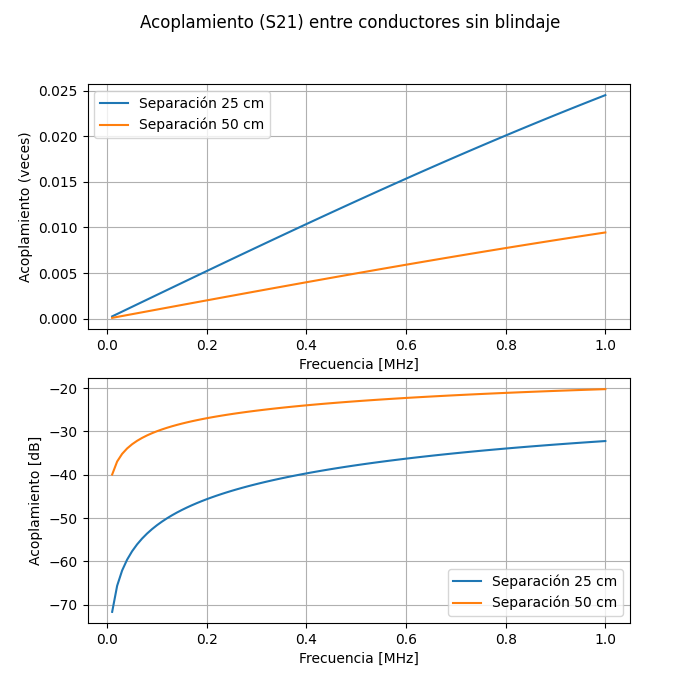
\includegraphics[width=0.47\linewidth]{imagenes/acoplamiento_sin_blindaje_resultados_bajas.png}
  \caption{Acoplamiento sin blindaje para bajas frecuencias.}%
  \label{fig:imagenes/acoplamiento_sin_blindaje_resultados_bajas}
\end{figure}

\begin{figure}[ht]
  \centering
  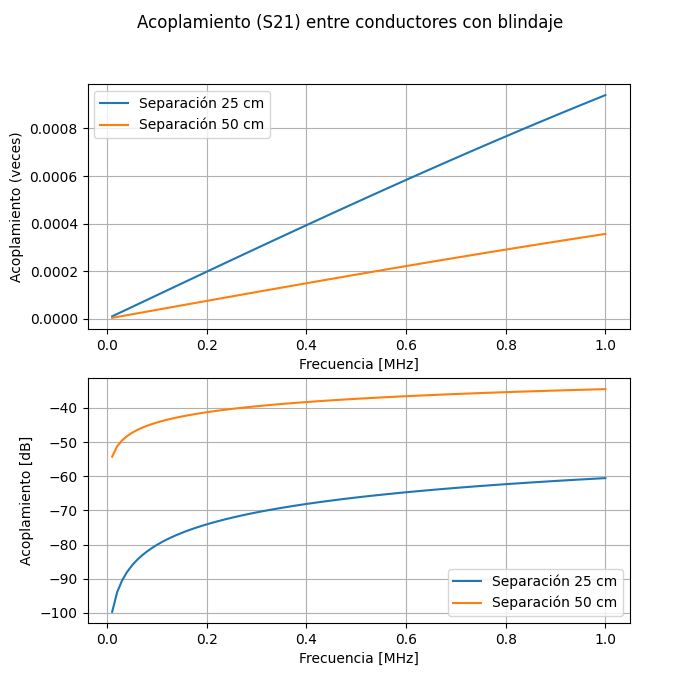
\includegraphics[width=0.47\linewidth]{imagenes/acoplamiento_con_blindaje_resultados_bajas.png}
  \caption{Acoplamiento con blindaje para bajas frecuencias.}%
  \label{fig:imagenes/acoplamiento_con_blindaje_resultados_bajas}
\end{figure}

\begin{figure}[ht]
  \centering
  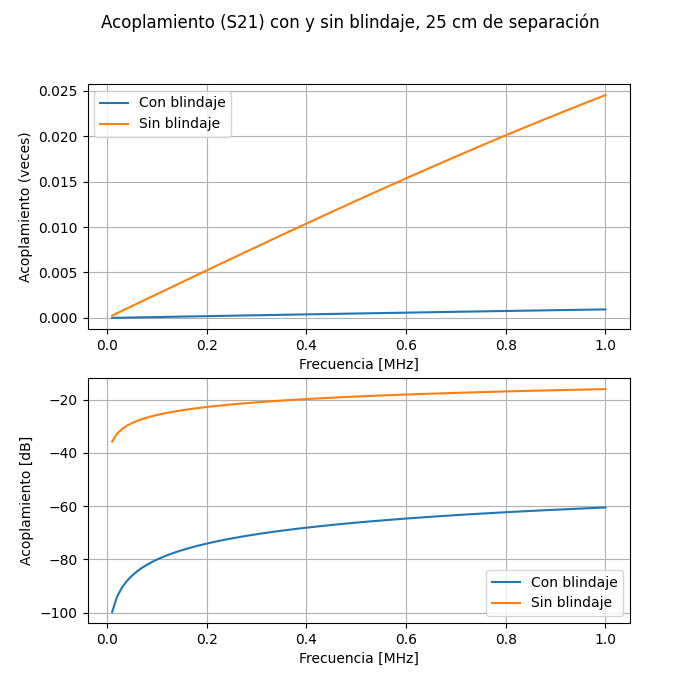
\includegraphics[width=0.6\linewidth]{imagenes/efecto_blindaje_25cm.png}
  \caption{Efecto del blindaje para una separación de \SI{25}{\cm}.}%
  \label{fig:imagenes/efecto_blindaje_25cm}
\end{figure}

\begin{figure}[ht]
  \centering
  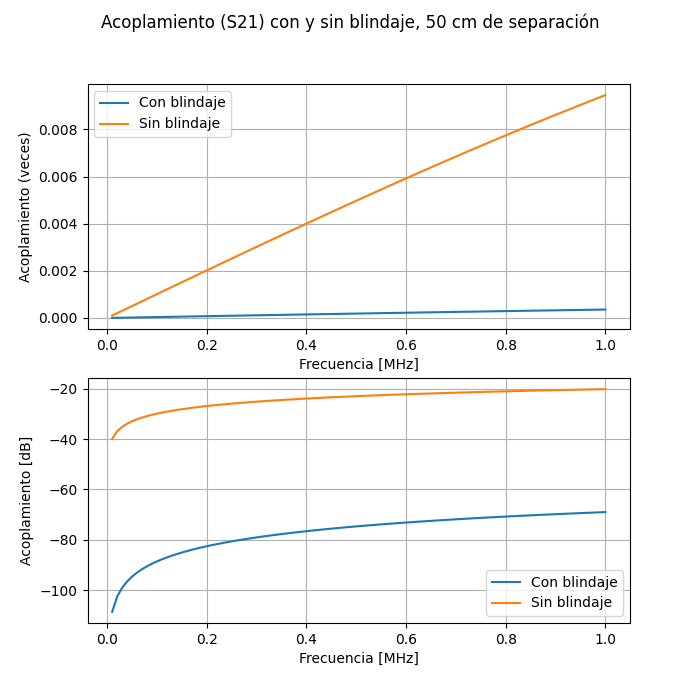
\includegraphics[width=0.6\linewidth]{imagenes/efecto_blindaje_50cm.png}
  \caption{Efecto del blindaje para una separación de \SI{50}{\cm}.}%
  \label{fig:imagenes/efecto_blindaje_50cm}
\end{figure}

\begin{figure}[ht]
  \centering
  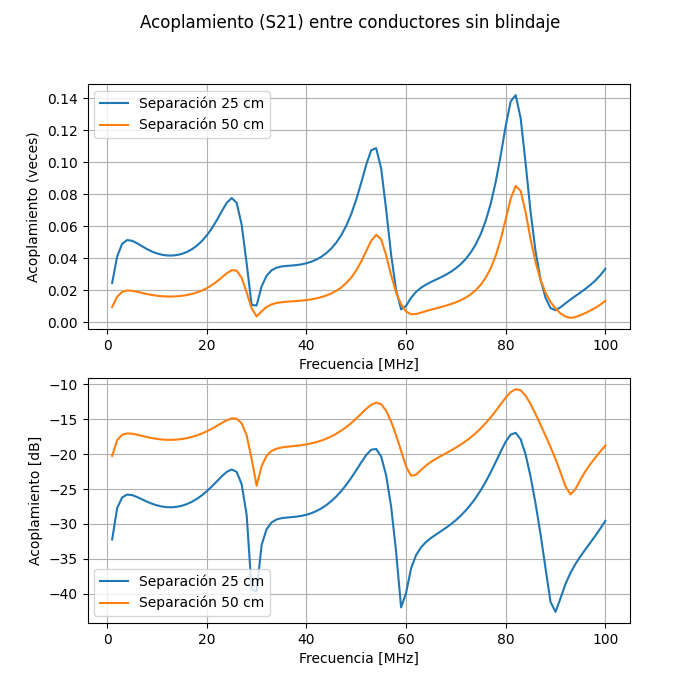
\includegraphics[width=0.6\linewidth]{imagenes/acoplamiento_sin_blindaje_resultados_altas.png}
  \caption{Acoplamiento sin blindaje para altas frecuencias.}%
  \label{fig:imagenes/acoplamiento_sin_blindaje_resultados_altas}
\end{figure}

\begin{figure}[ht]
  \centering
  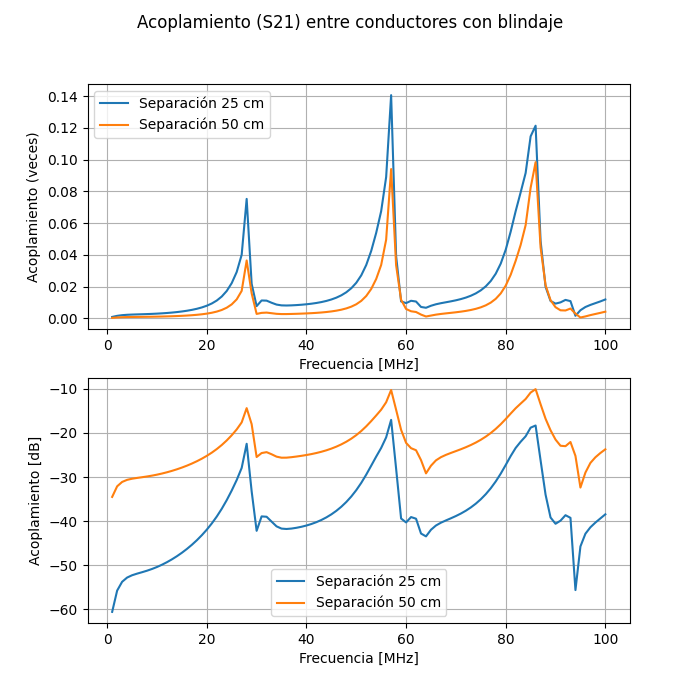
\includegraphics[width=0.6\linewidth]{imagenes/acoplamiento_con_blindaje_resultados_altas.png}
  \caption{Acoplamiento con blindaje para altas frecuencias.}%
  \label{fig:imagenes/acoplamiento_con_blindaje_resultados_altas}
\end{figure}
